\chapter{Implementasi dan Pengujian}
\label{chap:implementasipengujian}

\section{Implementasi}
\label{sec:implementasi}

\subsection{Lingkungan Implementasi}
\label{sec:lingkunganimplementasi}
Impelementasi dilakukan dengan menggunakan laptop peneliti. Berikut adalah spesifikasi laptop peneliti:
\begin{enumerate}
	\item Processor: Intel(R) Core(TM)2 Duo 2.40 GHz
	\item RAM: 2048 MB
	\item Sistem Operasi: Windows 7 Ultimate 32-bit (6.1, Build 7601)
	\item Versi Java: 1.8.0\_91
	\item Versi Play Framework: 2.4.3
	\item Browser: Google Chrome
\end{enumerate}

\subsection{Hasil Implementasi}
\label{sec:hasilimplementasi}
Hasil implementasi dari penelitian ini adalah aplikasi berbasis \textit{web} yang menggunakan Play Framework. Aplikasi dapat diakses ke jaringan lokal milik peneliti melalui URL \url{http://localhost/bukitjarian/}. Aplikasi KIRI \textit{Dashboard} terbagi ke dalam 16 bagian.
\begin{enumerate}
	\item \textbf{Bagian \textit{Register}}\\
	Bagian ini merupakan bagian untuk mendaftarkan pengguna baru ke dalam sistem KIRI. Pengguna dapat mengisi alamat \textit{email}, nama lengkap, dan nama perusahaan pada formulir registrasi (Gambar \ref{fig:5_register_1}). Jika pendaftaran berhasil (Gambar \ref{fig:5_register_2}), pengguna dapat langsung mengecek kotak masuk \textit{email} yang didaftarkan (Gambar \ref{fig:5_register_3}).

	\begin{figure}[htbp]
		\centering
			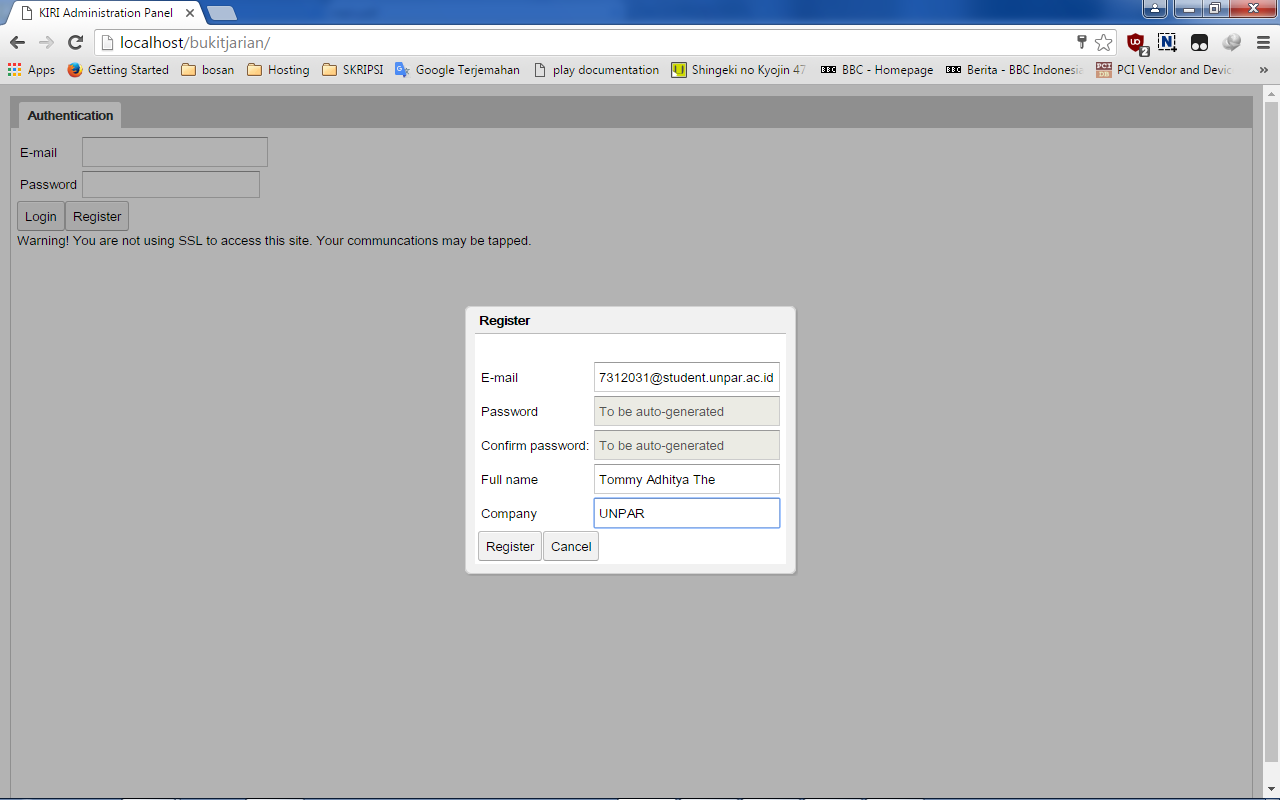
\includegraphics[scale=0.45]{Gambar/5_register_1.png}
		\caption{Formulir registrasi}
		\label{fig:5_register_1}
	\end{figure}

	\begin{figure}[htbp]
		\centering
			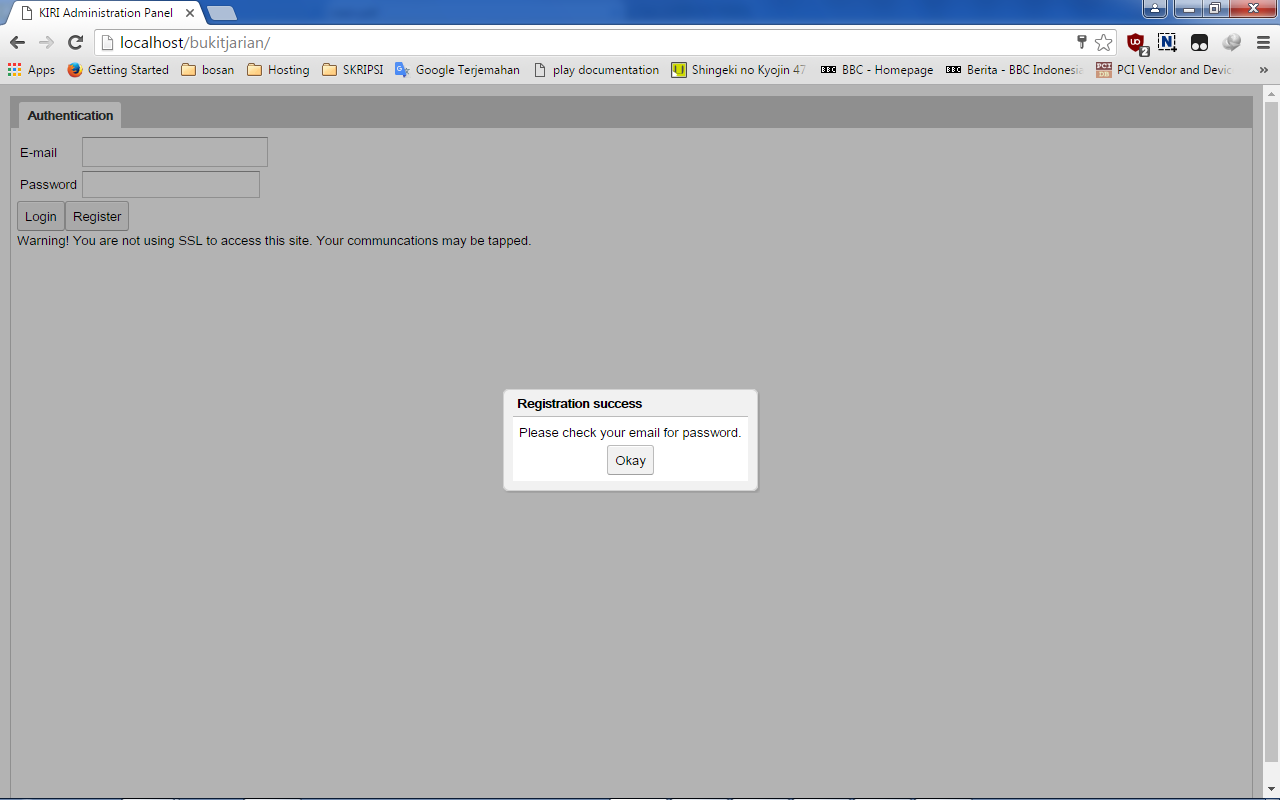
\includegraphics[scale=0.45]{Gambar/5_register_2.png}
		\caption{Registrasi berhasil}
		\label{fig:5_register_2}
	\end{figure}

	\begin{figure}[htbp]
		\centering
			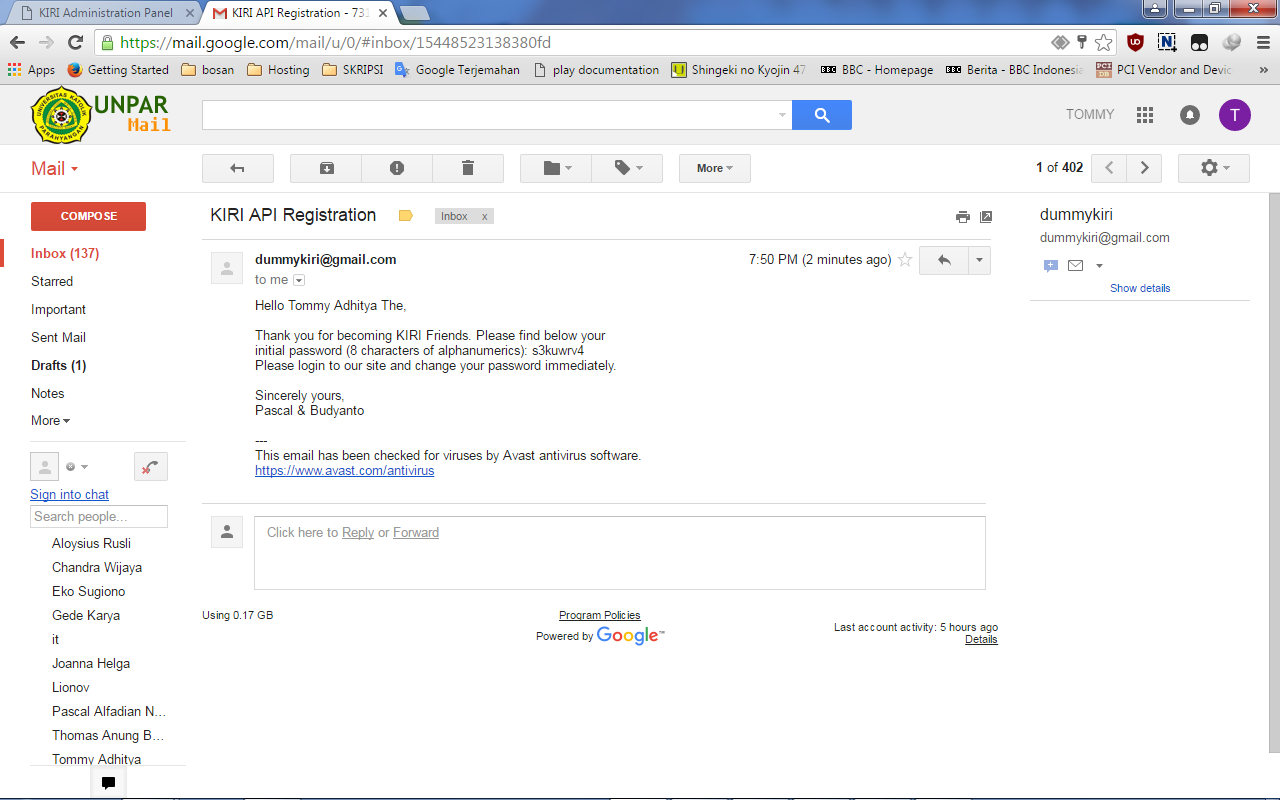
\includegraphics[scale=0.45]{Gambar/5_register_3.png}
		\caption{Kotak masuk \textit{email} pengguna}
		\label{fig:5_register_3}
	\end{figure}

	\item \textbf{Bagian \textit{Login}}\\
	Bagian ini merupakan bagian untuk masuk ke dalam sistem KIRI \textit{Dashboard} sebagai pengguna yang terdaftar. Jika \textit{email} pengguna terdaftar dan sandi yang pengguna masukkan sesuai, maka pengguna akan mendapatkan akses masuk KIRI \textit{Dashboard} (Gambar \ref{fig:5_login}).

	\begin{figure}[htbp]
		\centering
			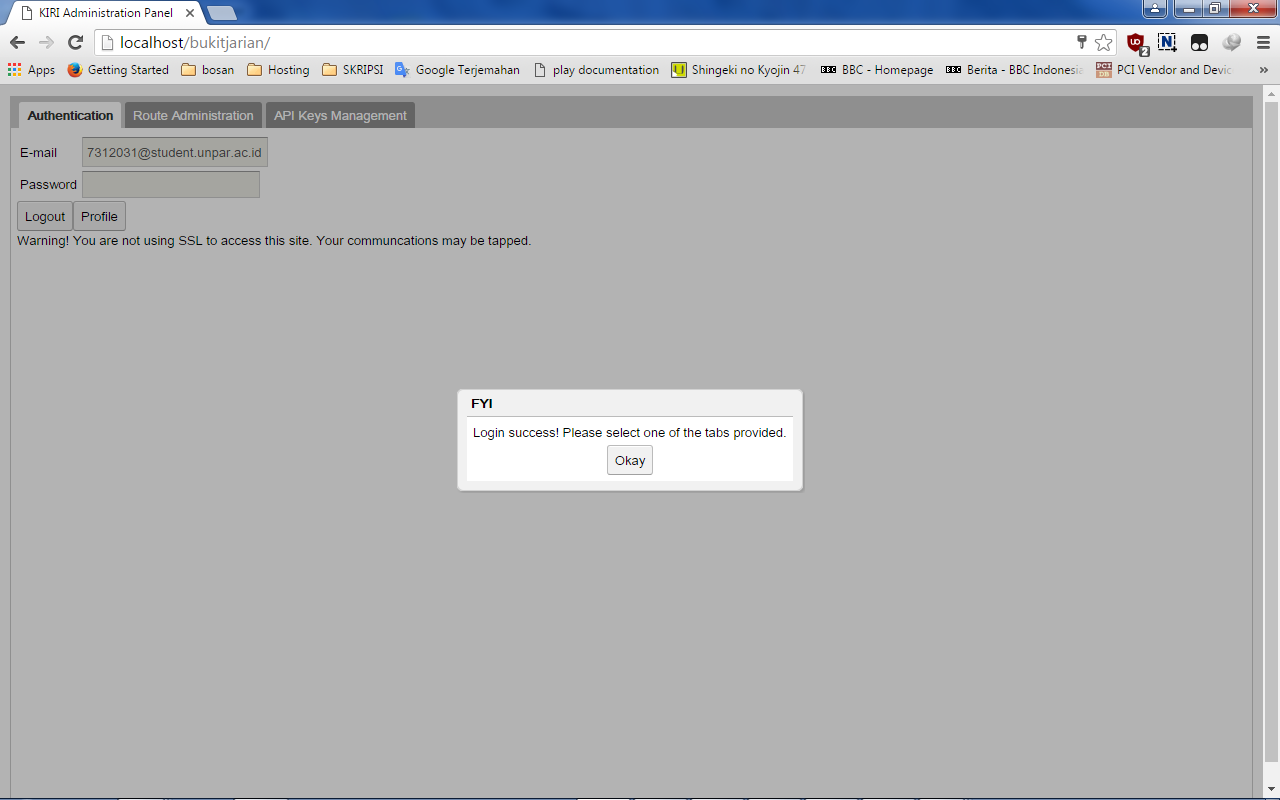
\includegraphics[scale=0.45]{Gambar/5_login.png}
		\caption{\textit{Login} dengan \textit{email} pengguna}
		\label{fig:5_login}
	\end{figure}

	\item \textbf{Bagian Pemeriksaan \textit{Login}}\\
	Bagian ini merupakan bagian pemberi hak akses rute dan API \textit{keys} kepada pengguna. Jika \textit{email} pengguna yang terdaftar memiliki hak akses terhadap rute dan API \textit{keys}, maka tampilan pengelola rute dan pengelola API \textit{keys} akan ditampilkan di layar (Gambar \ref{fig:5_login}).
	
	\item \textbf{Bagian Melihat Data Pribadi Pengguna}\\
	Bagian ini merupakan bagian yang akan menampilkan data pribadi pengguna. Data pribadi yang ditampilkan adalah nama lengkap dan nama perusahaan pengguna (Gambar \ref{fig:5_getprofil}).

	\begin{figure}[htbp]
		\centering
			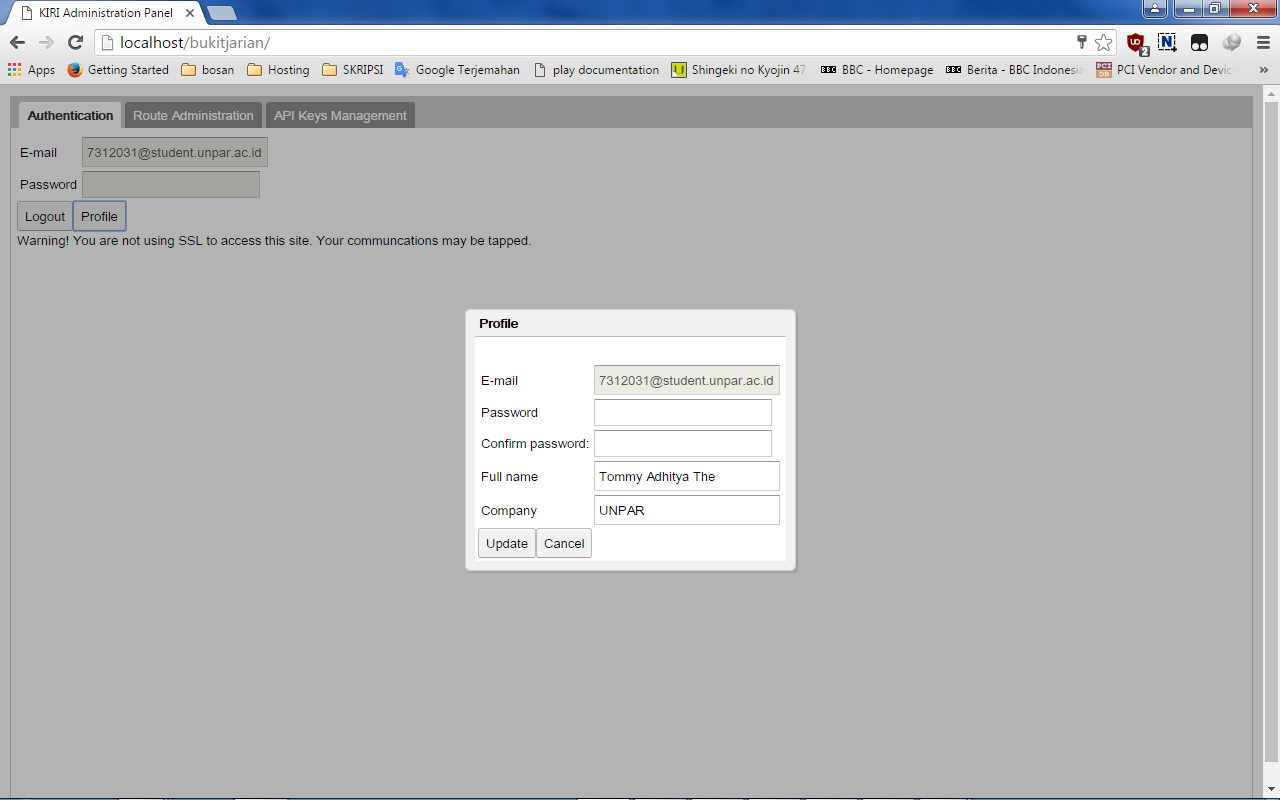
\includegraphics[scale=0.45]{Gambar/5_getprofil.png}
		\caption{Melihat data pribadi pengguna}
		\label{fig:5_getprofil}
	\end{figure}

	\item \textbf{Bagian Mengubah Data Pribadi Pengguna}\\
	Bagian ini merupakan bagian untuk mengubah data pribadi pengguna. Pengguna mengisi formulir untuk nama lengkap, nama perusahaan, dan sandi (Gambar \ref{fig:5_updateprofile_1}). Jika formulir memenuhi persyaratan sistem, maka akan muncul pesan keberhasilan (Gambar \ref{fig:5_updateprofile_2}).

	\begin{figure}[htbp]
		\centering
			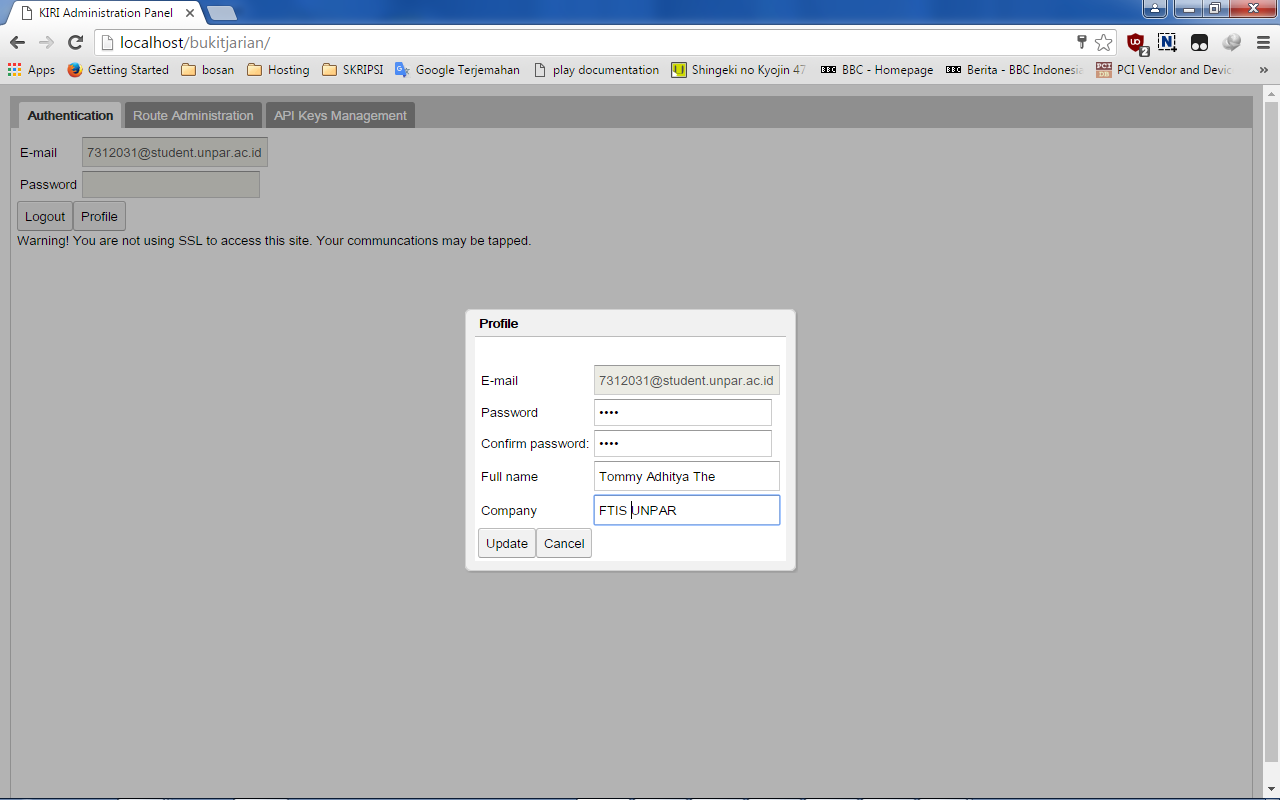
\includegraphics[scale=0.45]{Gambar/5_updateprofile_1.png}
		\caption{Formulir ubah data pribadi pengguna}
		\label{fig:5_updateprofile_1}
	\end{figure}

	\begin{figure}[htbp]
		\centering
			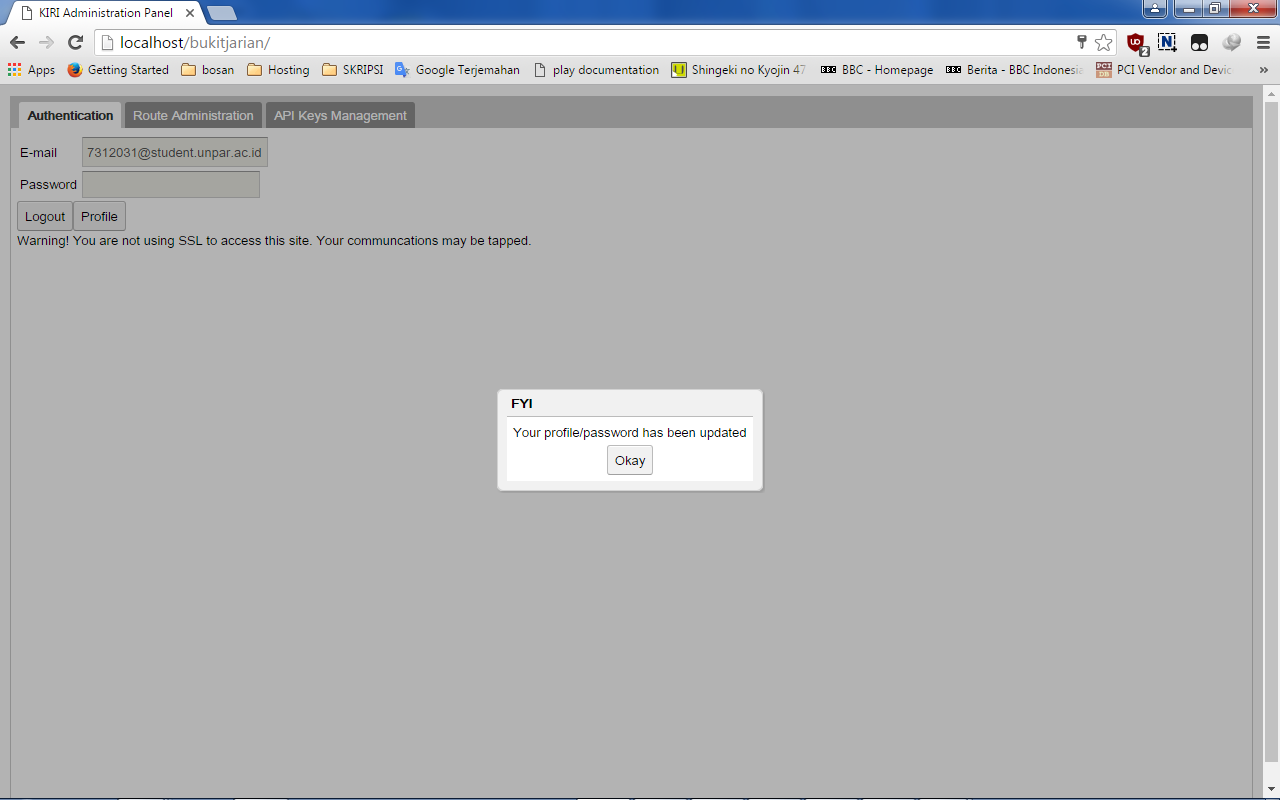
\includegraphics[scale=0.45]{Gambar/5_updateprofile_2.png}
		\caption{Ubah data pribadi pengguna berhasil}
		\label{fig:5_updateprofile_2}
	\end{figure}

	\item \textbf{Bagian Melihat Daftar API \textit{Keys}}\\
	Bagian ini merupakan bagian yang akan menampilkan daftar API \textit{keys} yang dimiliki oleh pengguna. Pengguna yang baru mendaftarkan diri belum memiliki API \textit{key} (Gambar \ref{fig:5_apikey}).

	\begin{figure}[htbp]
		\centering
			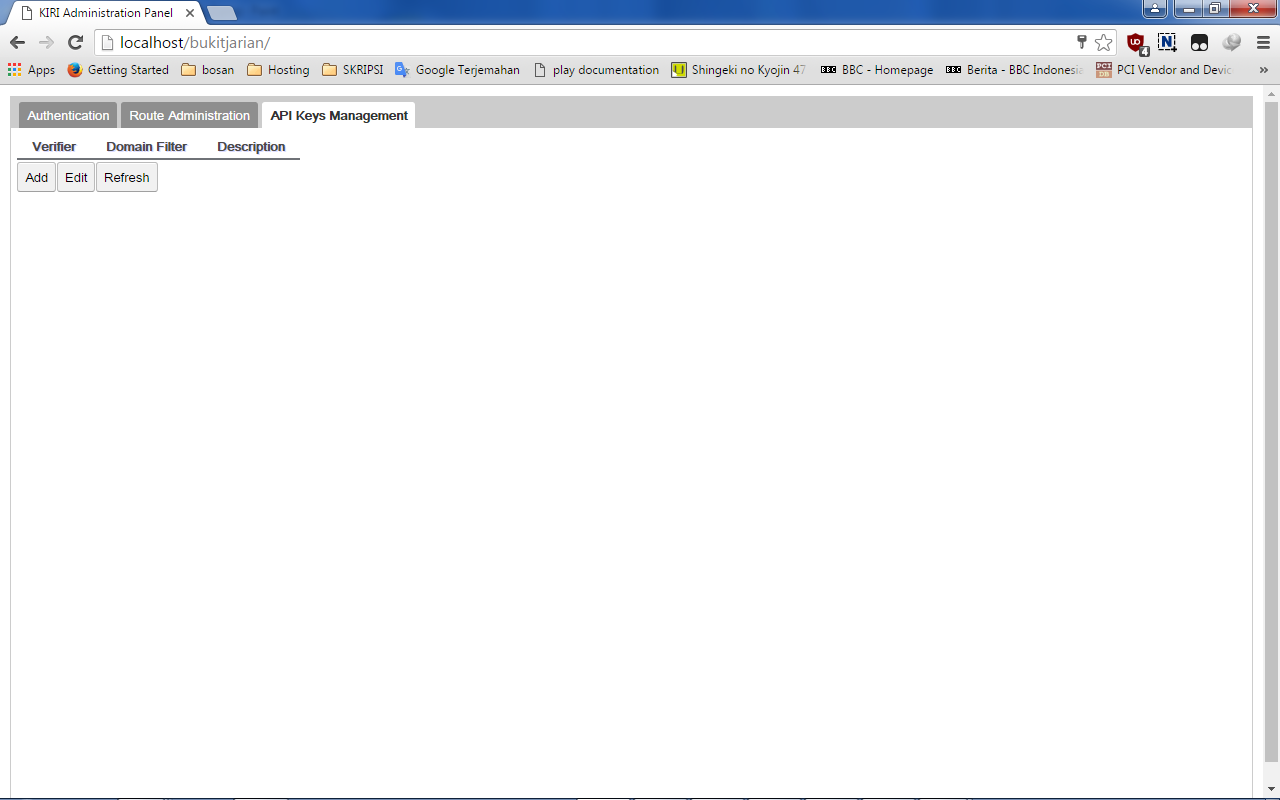
\includegraphics[scale=0.45]{Gambar/5_apikey.png}
		\caption{Daftar API \textit{keys} pengguna}
		\label{fig:5_apikey}
	\end{figure}

	\item \textbf{Bagian Menambahkan API \textit{Key}}\\
	Bagian ini merupakan bagian untuk menambahkan sebuah API \textit{key} ke dalam daftar milik pengguna. Pengguna mengisi formulir untuk nama \textit{domain} dan deskripsi mengenai API \textit{key} yang ingin ditambahkan (Gambar \ref{fig:5_addapikey_1}). Sistem KIRI akan membangun sebuah API \textit{key} baru secara acak (Gambar \ref{fig:5_addapikey_2}).

	\begin{figure}[htbp]
		\centering
			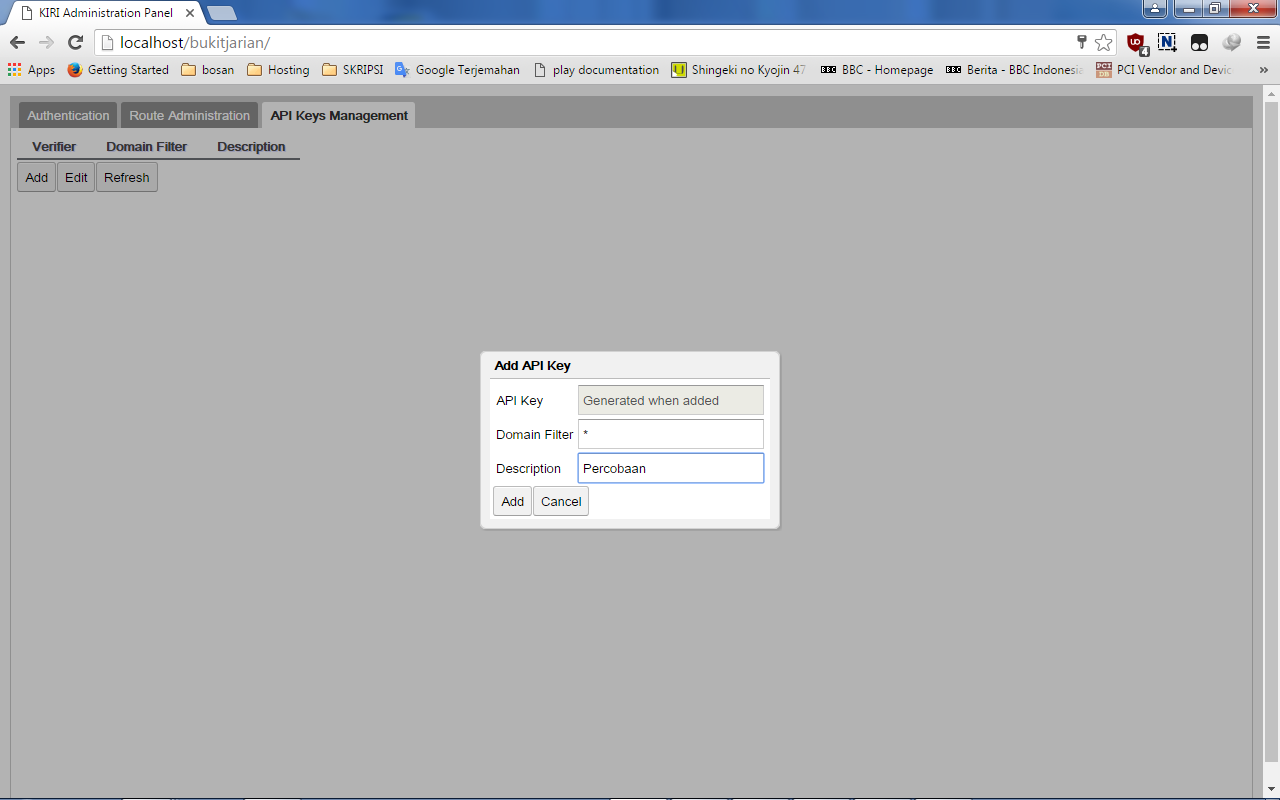
\includegraphics[scale=0.45]{Gambar/5_addapikey_1.png}
		\caption{Formulir untuk menambahkan API \textit{key}}
		\label{fig:5_addapikey_1}
	\end{figure}

	\begin{figure}[htbp]
		\centering
			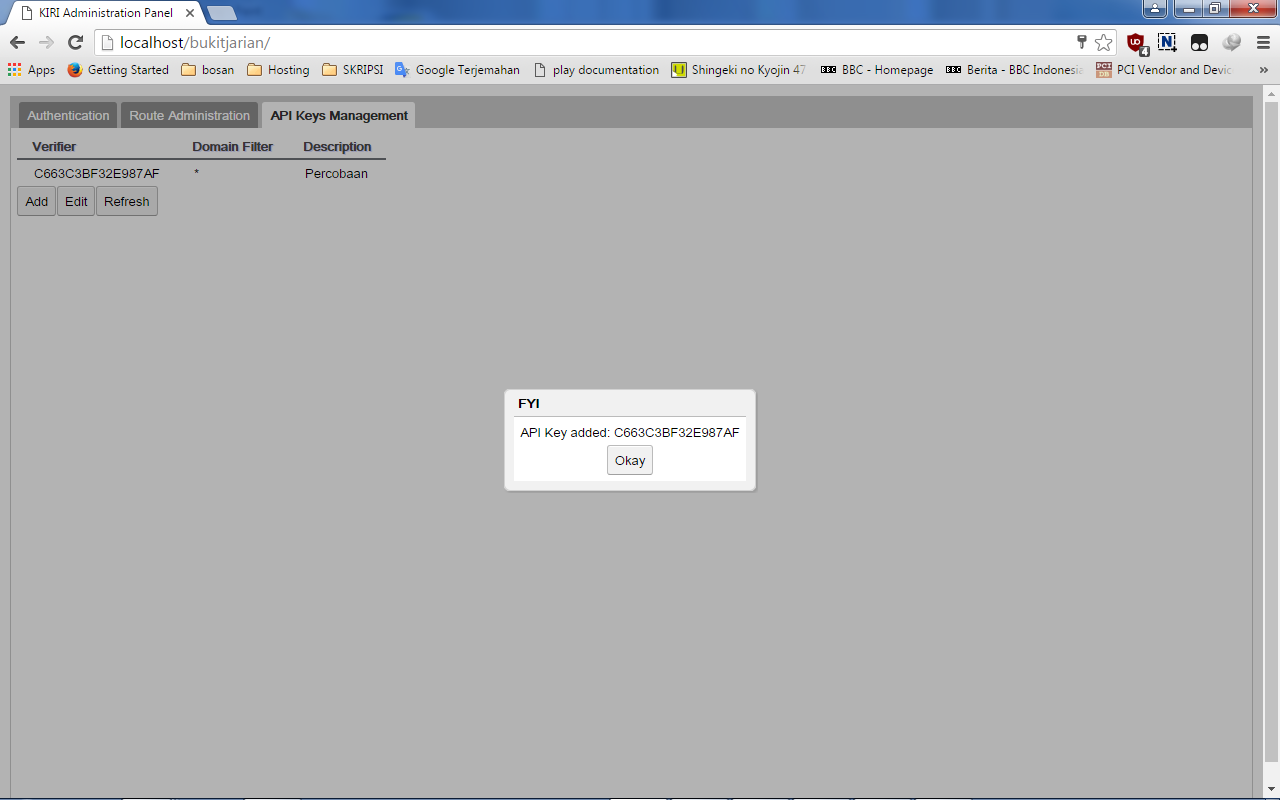
\includegraphics[scale=0.45]{Gambar/5_addapikey_2.png}
		\caption{API \textit{key} berhasil ditambahkan} 
		\label{fig:5_addapikey_2}
	\end{figure}

	\item \textbf{Bagian Mengubah API \textit{Key}}\\
	Bagian ini merupakan bagian untuk mengubah sebuah data API \textit{key} milik pengguna. Pengguna mengisi formulir untuk nama \textit{domain} dan deskripsi mengenai API \textit{key} yang ingin diubah (Gambar \ref{fig:5_editapikey_1}). Jika formulir memenuhi persyaratan sistem, maka akan muncul pesan keberhasilan (Gambar \ref{fig:5_editapikey_2}).

	\begin{figure}[htbp]
		\centering
			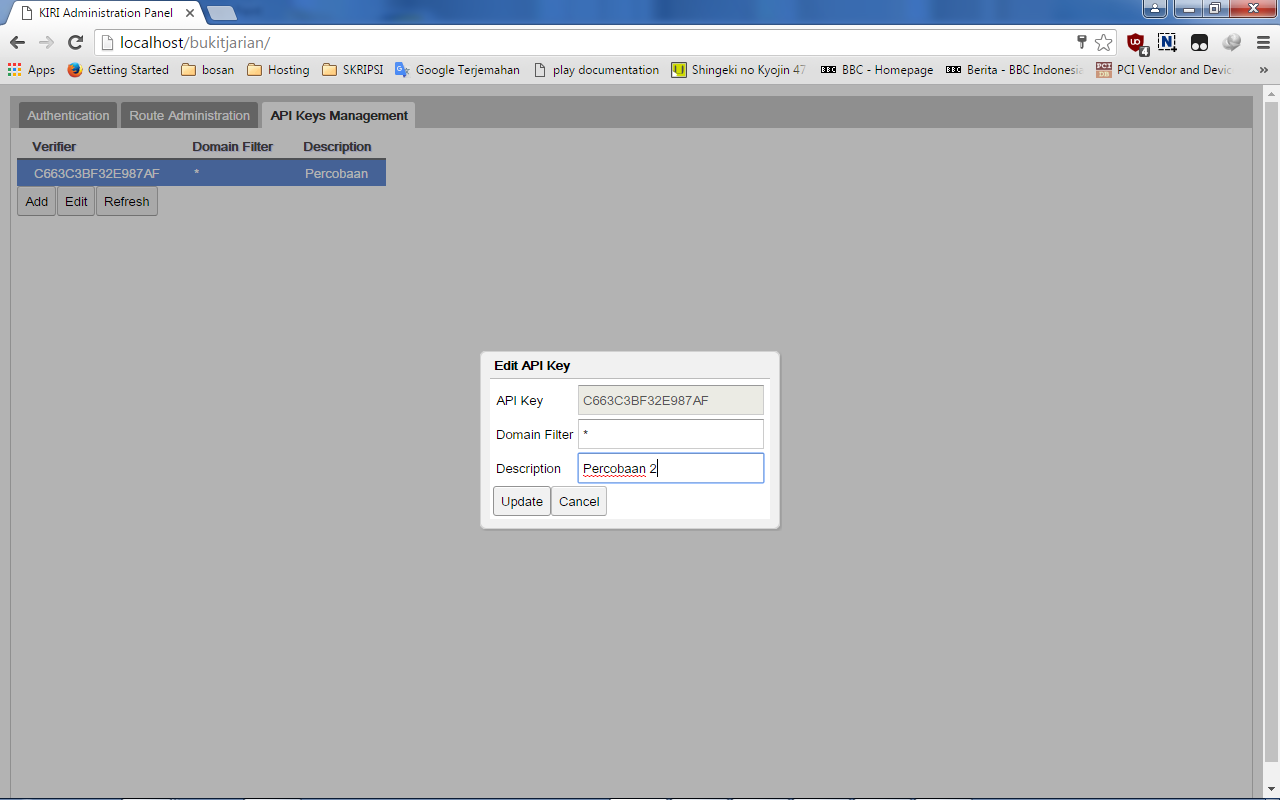
\includegraphics[scale=0.45]{Gambar/5_editapikey_1.png}
		\caption{Formulir untuk mengubah API \textit{key}}
		\label{fig:5_editapikey_1}
	\end{figure}

	\begin{figure}[htbp]
		\centering
			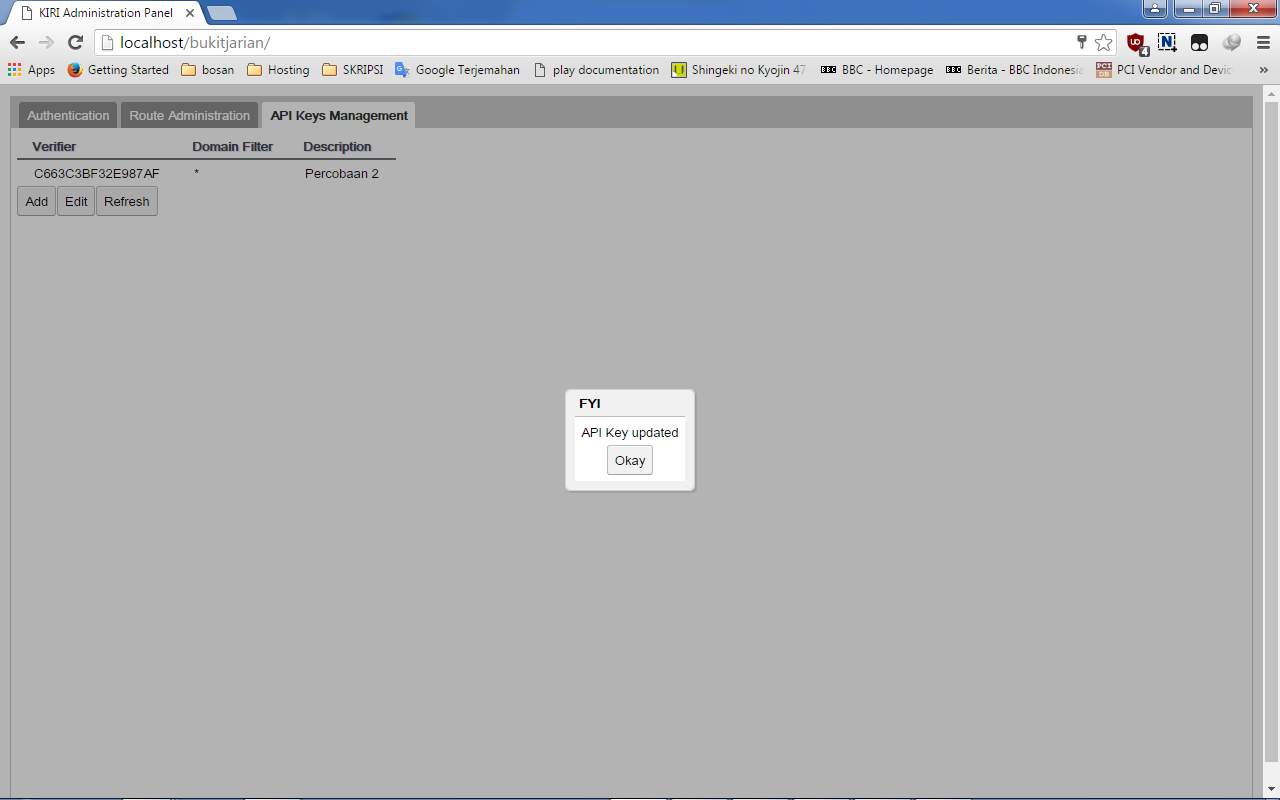
\includegraphics[scale=0.45]{Gambar/5_editapikey_2.png}
		\caption{Ubah data API \textit{key} berhasil} 
		\label{fig:5_editapikey_2}
	\end{figure}

	\item \textbf{Bagian Melihat Daftar Rute}\\
	Bagian ini merupakan bagian yang akan menampilkan daftar rute angkutan umum yang dimiliki oleh sistem KIRI (Gambar \ref{fig:5_gettracks}).

	\begin{figure}[htbp]
		\centering
			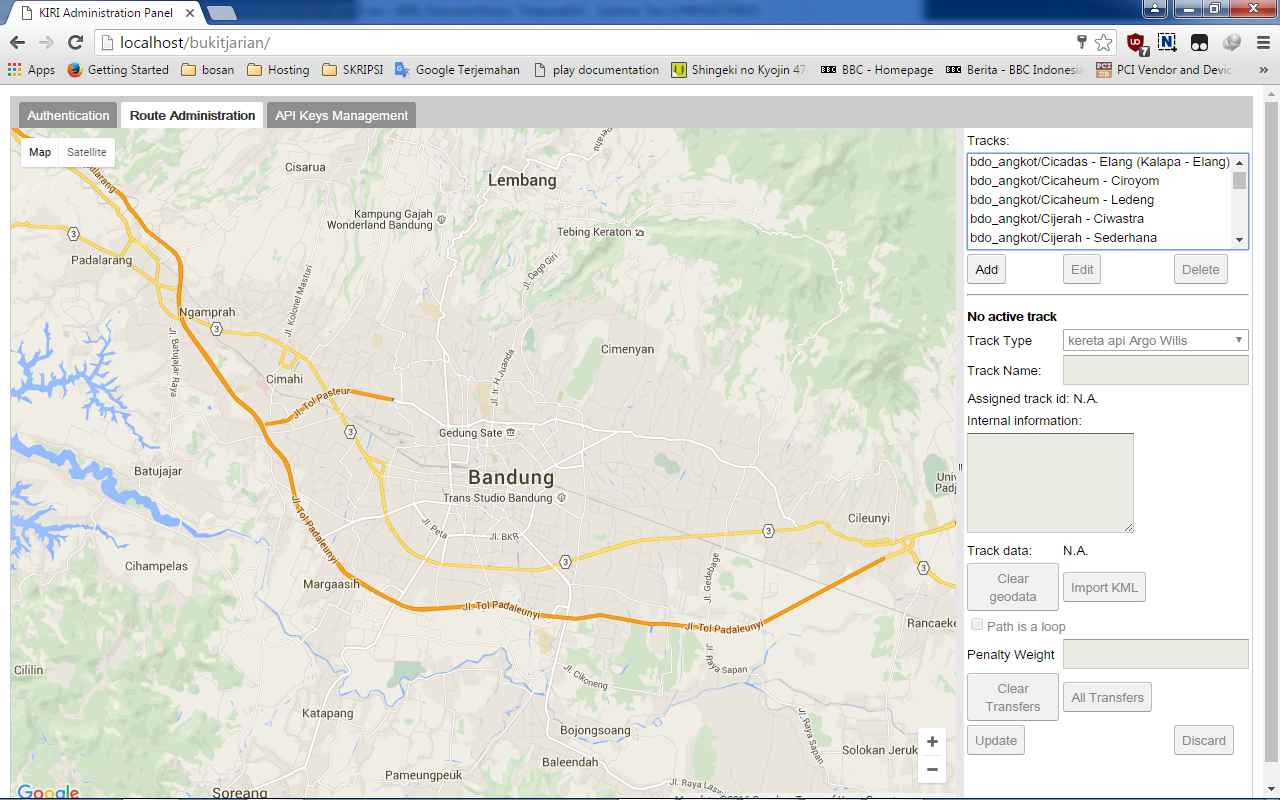
\includegraphics[scale=0.45]{Gambar/5_gettracks.png}
		\caption{Daftar rute angkutan umum sistem KIRI} 
		\label{fig:5_gettracks}
	\end{figure}

	\item \textbf{Bagian Melihat Informasi Rute secara Detail}\\
	Bagian ini merupakan bagian yang akan menampilkan detail data sebuah rute angkutan umum. Data yang ditampilkan adalah tipe angkutan umum, nama rute, informasi tambahan, data geografi dalam bentuk peta, informasi \textit{loop}, dan bobot pengali (Gambar \ref{fig:5_getdetailtrack}).

	\begin{figure}[htbp]
		\centering
			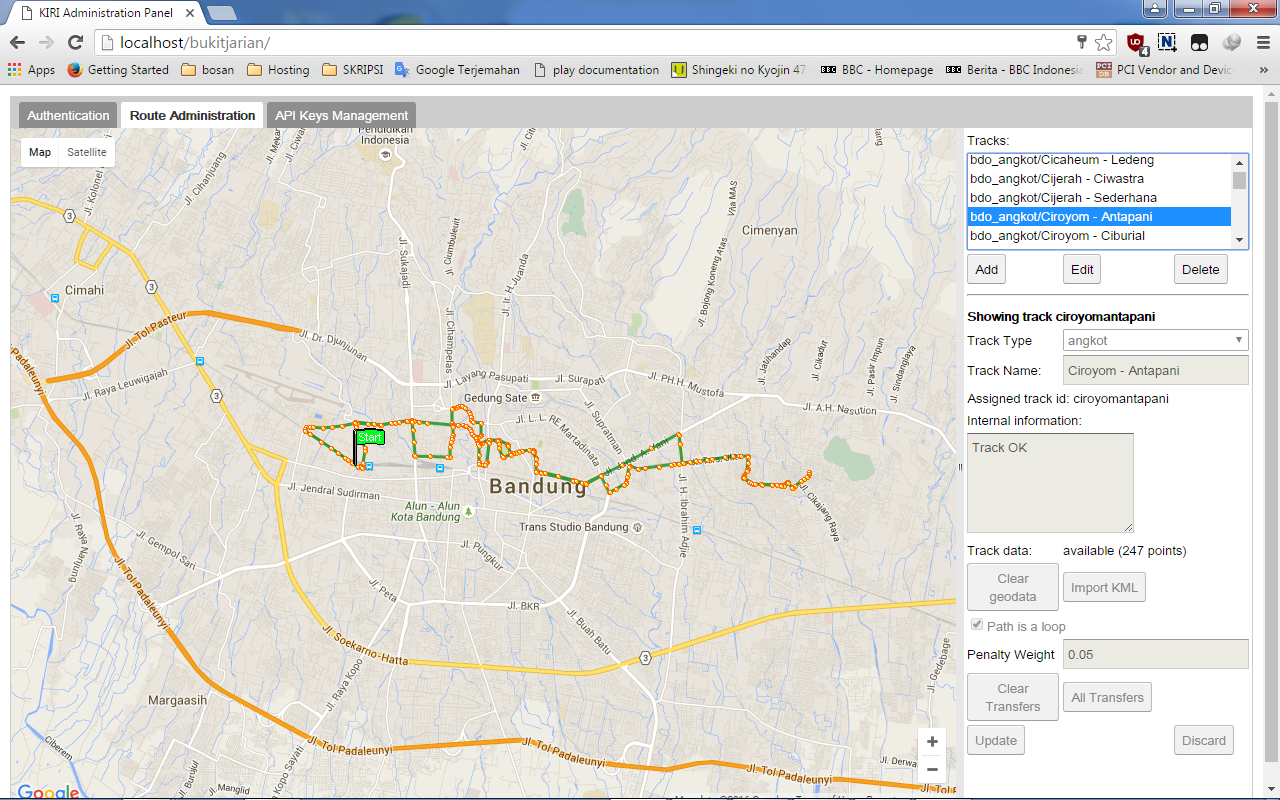
\includegraphics[scale=0.45]{Gambar/5_getdetailtrack.png}
		\caption{Detail rute angkutan umum Ciroyom-Antapani} 
		\label{fig:5_getdetailtrack}
	\end{figure}

	\item \textbf{Bagian Menambahkan Rute}\\
	Bagian ini merupakan bagian untuk menambahkan sebuah rute angkutan umum baru. Pengguna mengisi formulir untuk nama rute, informasi tambahan, bobot pengali rute, dan memilih jenis angkutan umum yang ingin ditambahkan (Gambar \ref{fig:5_addtrack_1}). Jika formulir memenuhi persyaratan sistem, maka akan rute baru akan muncul ke dalam daftar rute angkutan umum (Gambar \ref{fig:5_addtrack_2}).

	\begin{figure}[htbp]
		\centering
			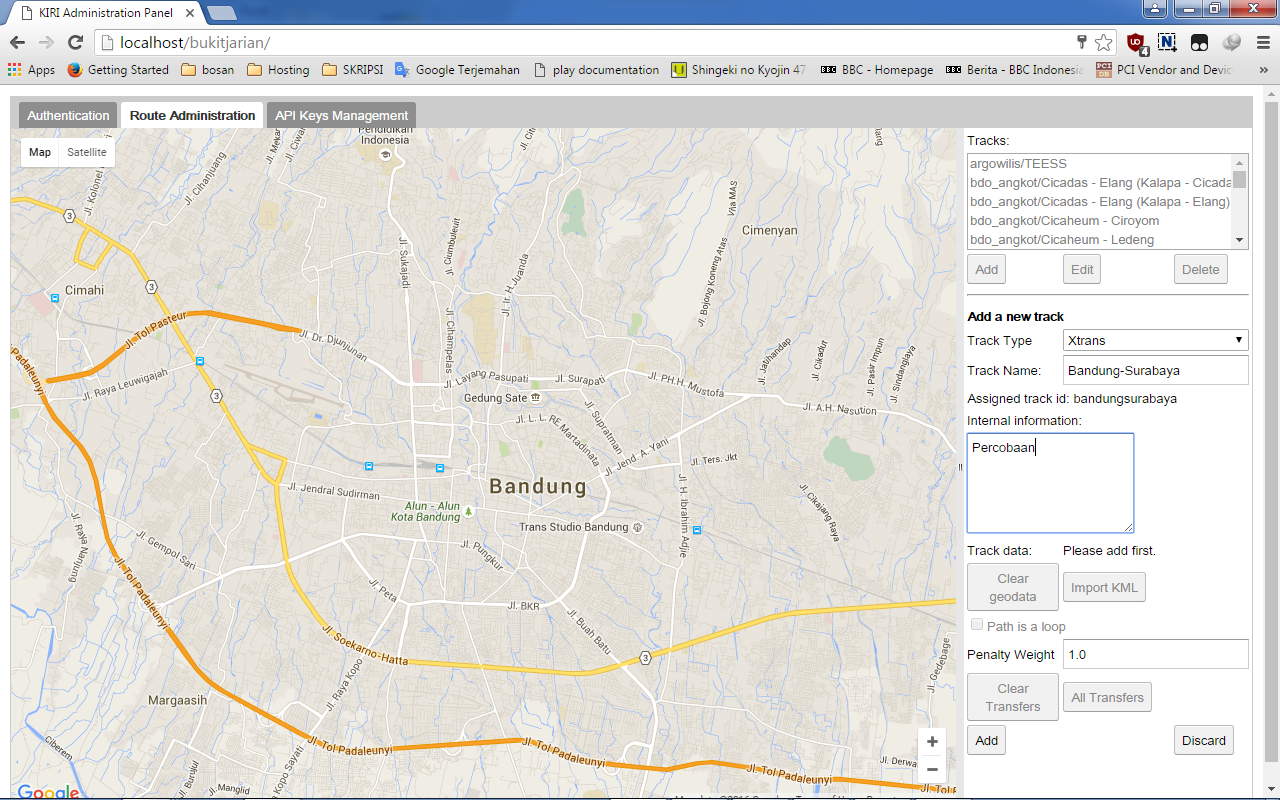
\includegraphics[scale=0.45]{Gambar/5_addtrack_1.png}
		\caption{Formulir penambahan rute angkutan umum} 
		\label{fig:5_addtrack_1}
	\end{figure}

	\begin{figure}[htbp]
		\centering
			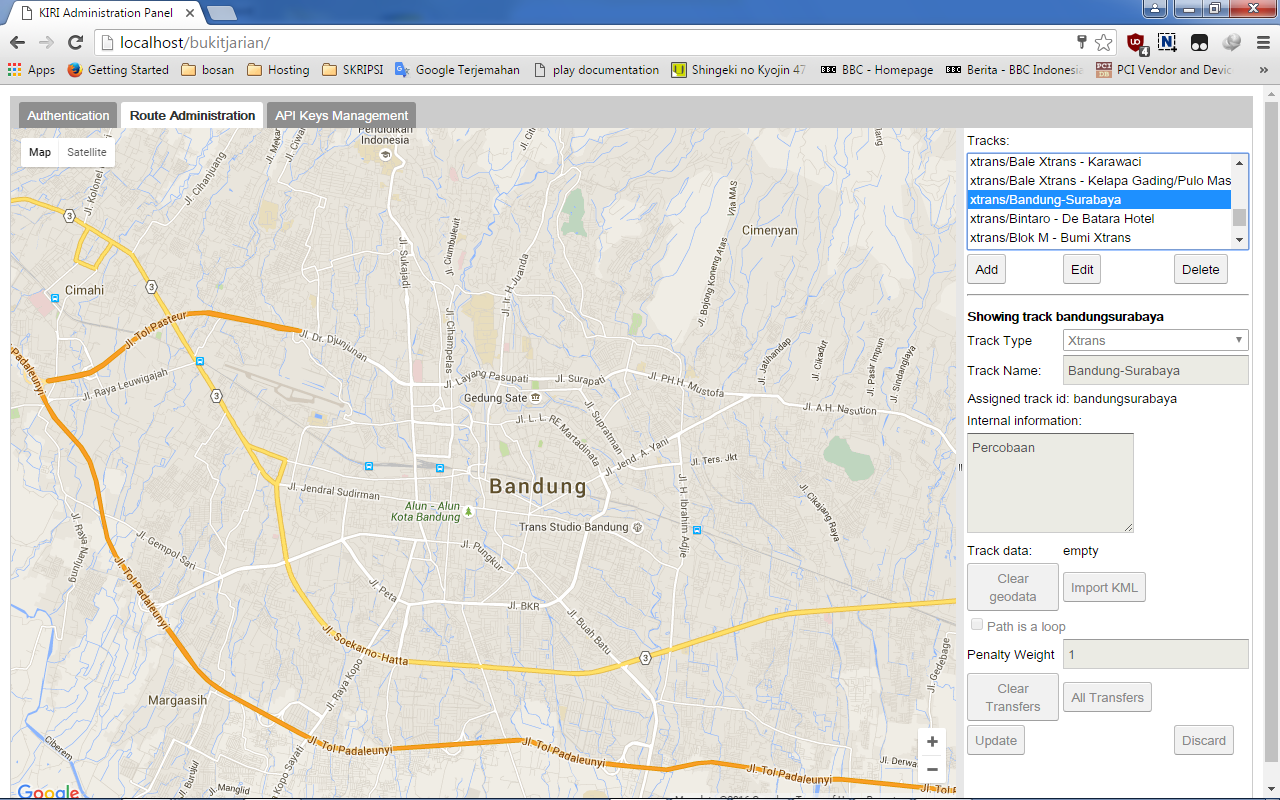
\includegraphics[scale=0.45]{Gambar/5_addtrack_2.png}
		\caption{Rute angkutan umum berhasil ditambahkan} 
		\label{fig:5_addtrack_2}
	\end{figure}

	\item \textbf{Bagian Mengubah Rute}\\
	Bagian ini merupakan bagian untuk mengubah data sebuah rute angkutan umum. Pengguna mengisi formulir untuk nama rute, informasi tambahan, bobot pengali rute, memilih jenis angkutan umum, dan memilih apakah terdapat \textit{loop} pada rute (Gambar \ref{fig:5_edittrack_1}). Jika formulir memenuhi persyaratan sistem, maka rute angkutan umum akan berubah (Gambar \ref{fig:5_edittrack_2}).

	\begin{figure}[htbp]
		\centering
			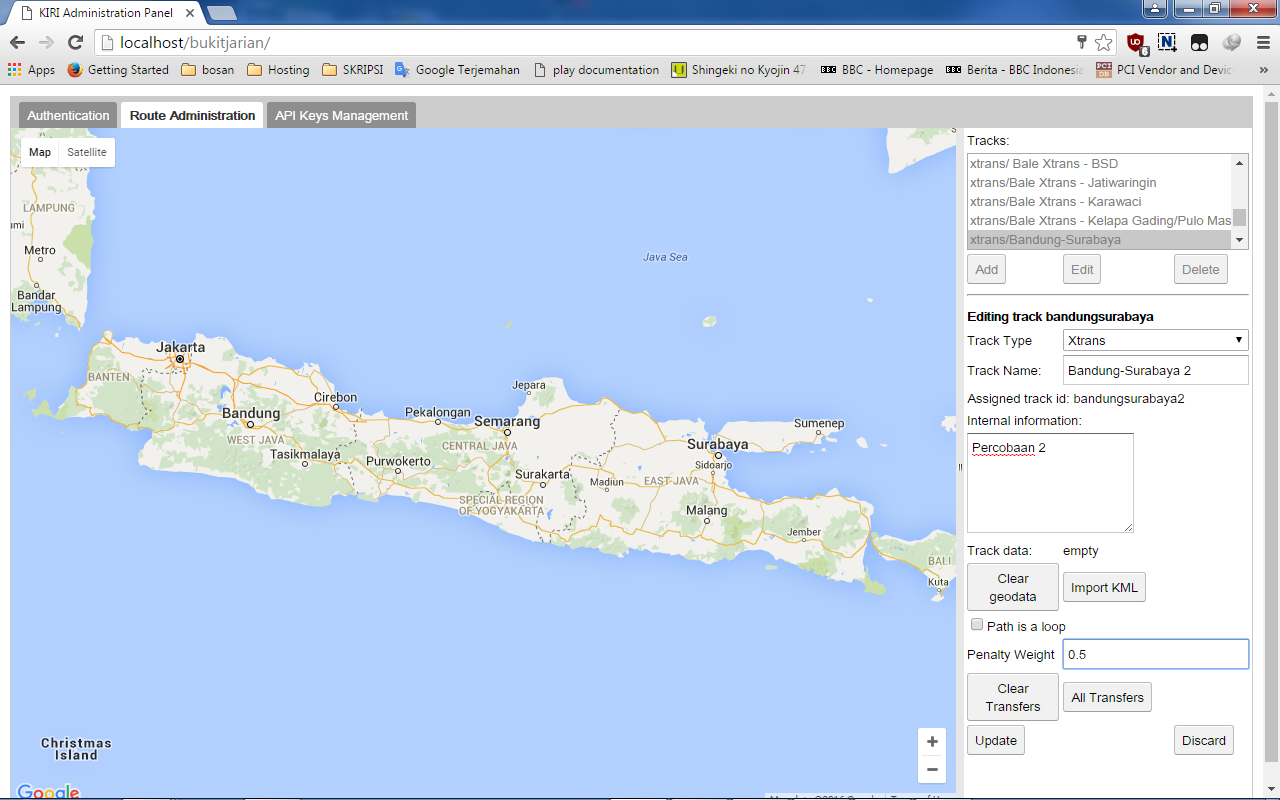
\includegraphics[scale=0.45]{Gambar/5_edittrack_1.png}
		\caption{Formulir mengubah data rute angkutan umum} 
		\label{fig:5_edittrack_1}
	\end{figure}

	\begin{figure}[htbp]
		\centering
			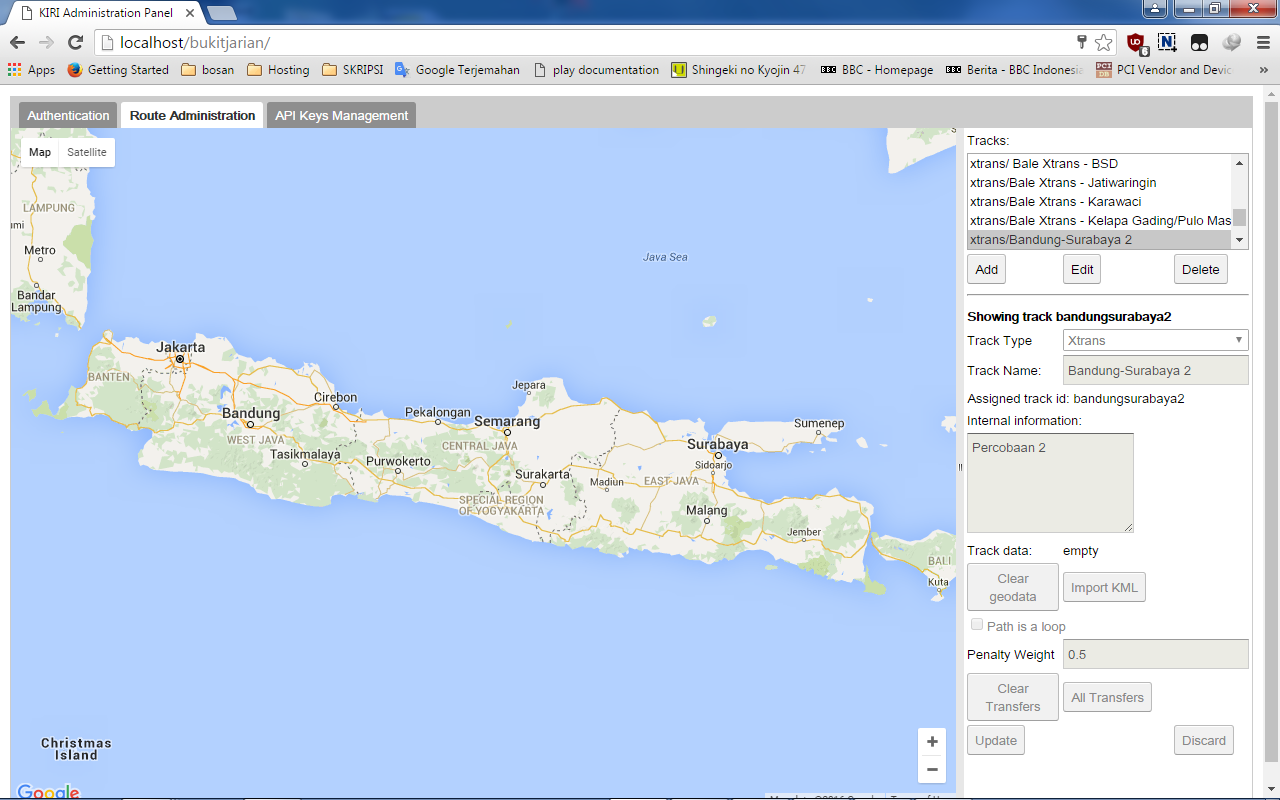
\includegraphics[scale=0.45]{Gambar/5_edittrack_2.png}
		\caption{Rute angkutan umum berhasil diubah} 
		\label{fig:5_edittrack_2}
	\end{figure}

	\item \textbf{Bagian Impor Data KML}\\
	Bagian ini merupakan bagian untuk menambahkan data geografi ke sebuah rute angkutan umum. Pengguna melakukan \textit{upload file} dalam format KML (Gambar \ref{fig:5_imporkml_1}). Jika \textit{file} memenuhi persyaratan sistem, maka akan muncul pesan keberhasilan dan peta akan berubah mengikuti data geografi pada \textit{file} tersebut (Gambar \ref{fig:5_imporkml_2}).

	\begin{figure}[htbp]
		\centering
			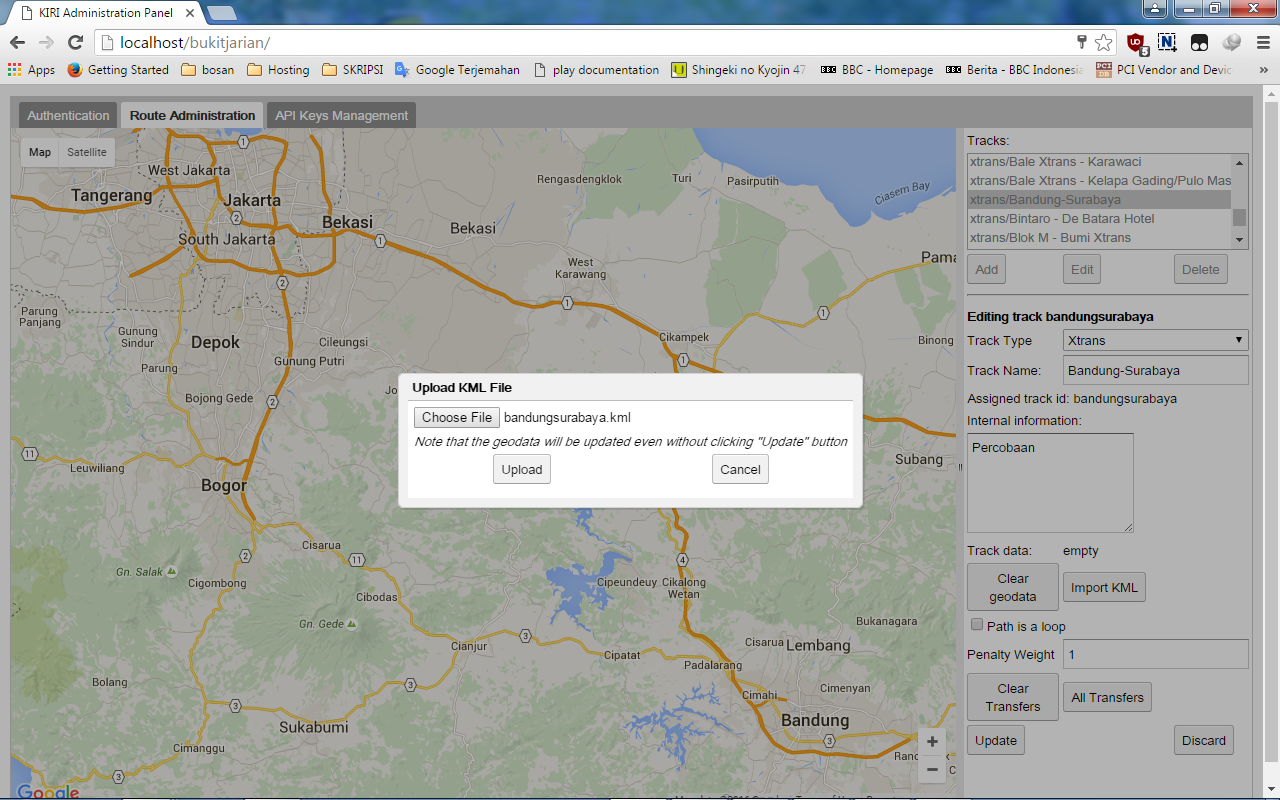
\includegraphics[scale=0.45]{Gambar/5_imporkml_1.png}
		\caption{\textit{Upload file} dalam format KML} 
		\label{fig:5_imporkml_1}
	\end{figure}

	\begin{figure}[htbp]
		\centering
			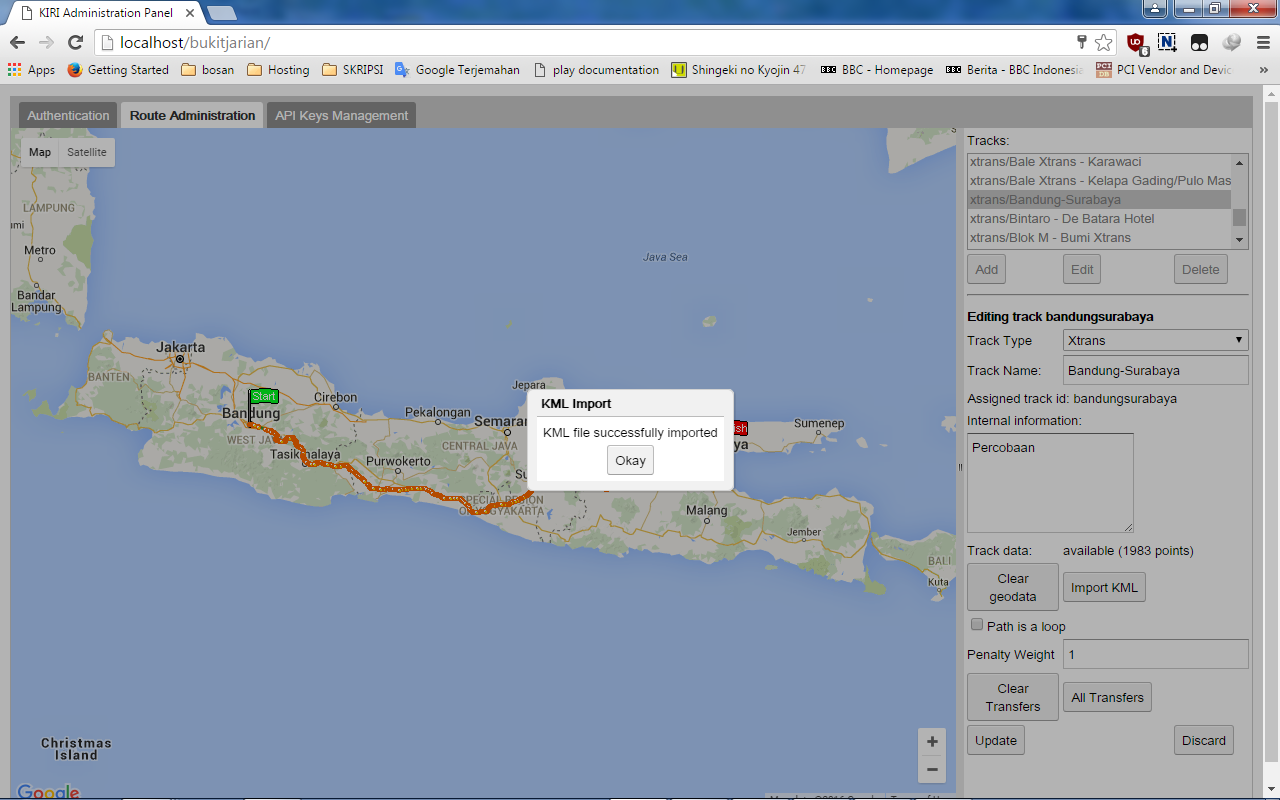
\includegraphics[scale=0.45]{Gambar/5_imporkml_2.png}
		\caption{Peta mengikuti data geografi \textit{file} yang di \textit{upload}} 
		\label{fig:5_imporkml_2}
	\end{figure}

	\item \textbf{Bagian Menghapus Data Geografis suatu Rute}\\
	Bagian ini merupakan bagian untuk menghapus data geografi sebuah rute angkutan umum. Pengguna melakukan verifikasi untuk menghapus data geografi suatu rute (Gambar \ref{fig:5_cleargeodata_1}). Data geografi pada peta terhapus (Gambar \ref{fig:5_cleargeodata_2}).

	\begin{figure}[htbp]
		\centering
			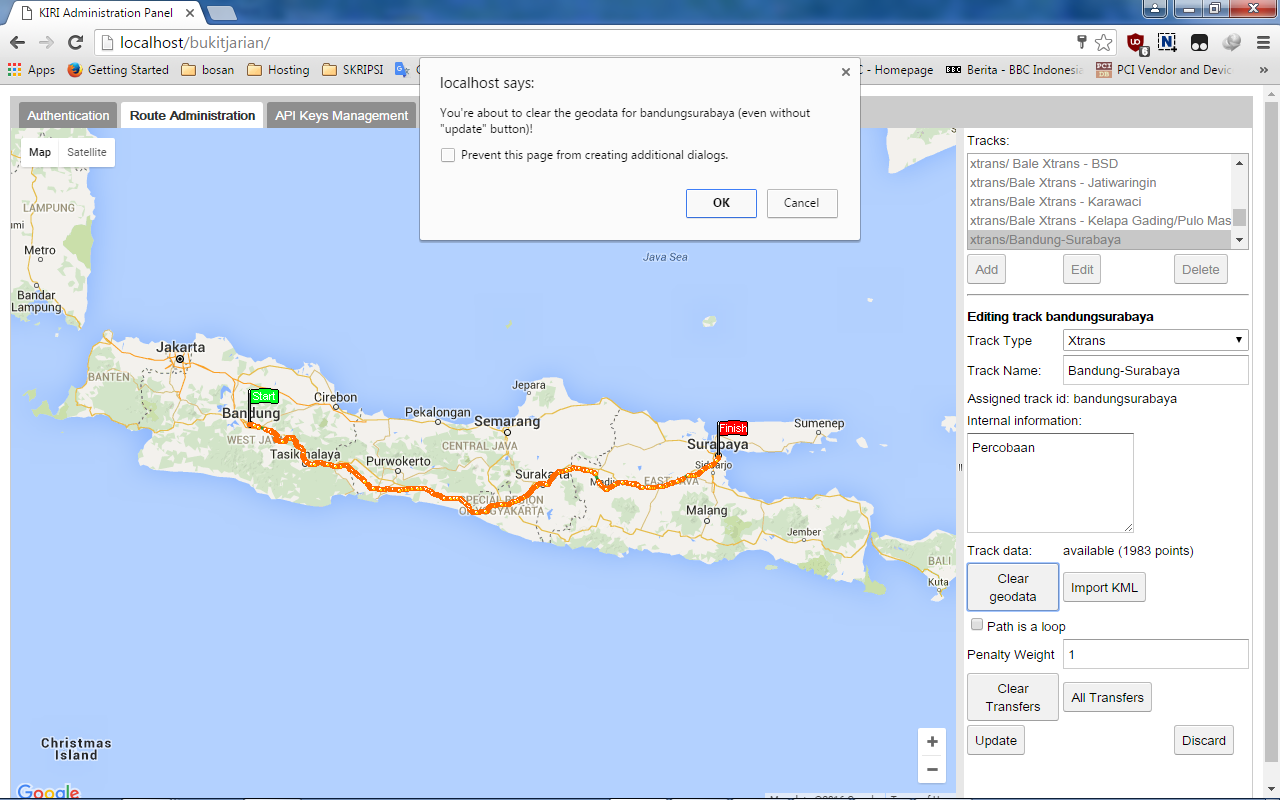
\includegraphics[scale=0.45]{Gambar/5_cleargeodata_1.png}
		\caption{Verifikasi penghapusan data geografi} 
		\label{fig:5_cleargeodata_1}
	\end{figure}

	\begin{figure}[htbp]
		\centering
			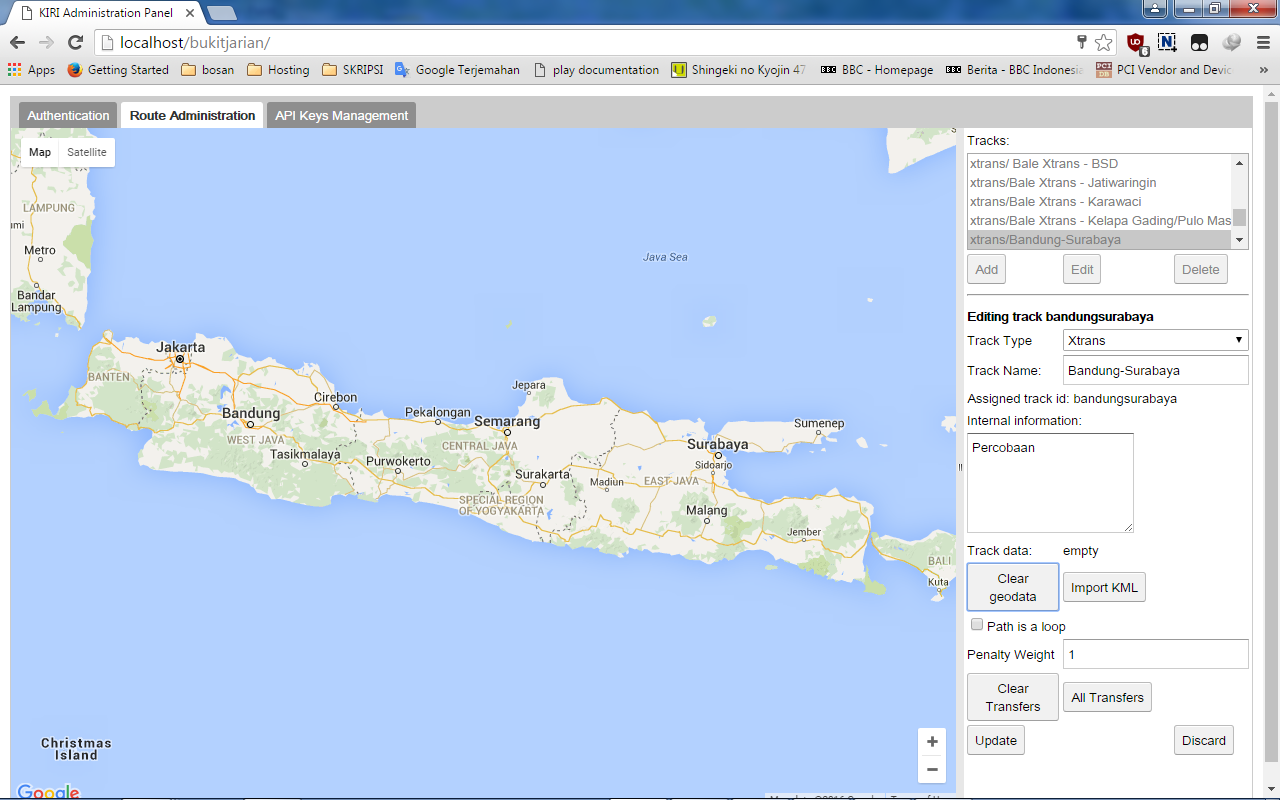
\includegraphics[scale=0.45]{Gambar/5_cleargeodata_2.png}
		\caption{Data geografi pada peta hilang} 
		\label{fig:5_cleargeodata_2}
	\end{figure}

	\item \textbf{Bagian Menghapus Rute}\\
	Bagian ini merupakan bagian untuk menghapus sebuah rute angkutan umum. Pengguna memilih dan melakukan verifikasi rute angkutan umum yang ingin dihapus (Gambar \ref{fig:5_deletetrack_1}). Rute angkutan umum terhapus dari sistem KIRI (Gambar \ref{fig:5_deletetrack_2}).

	\begin{figure}[htbp]
		\centering
			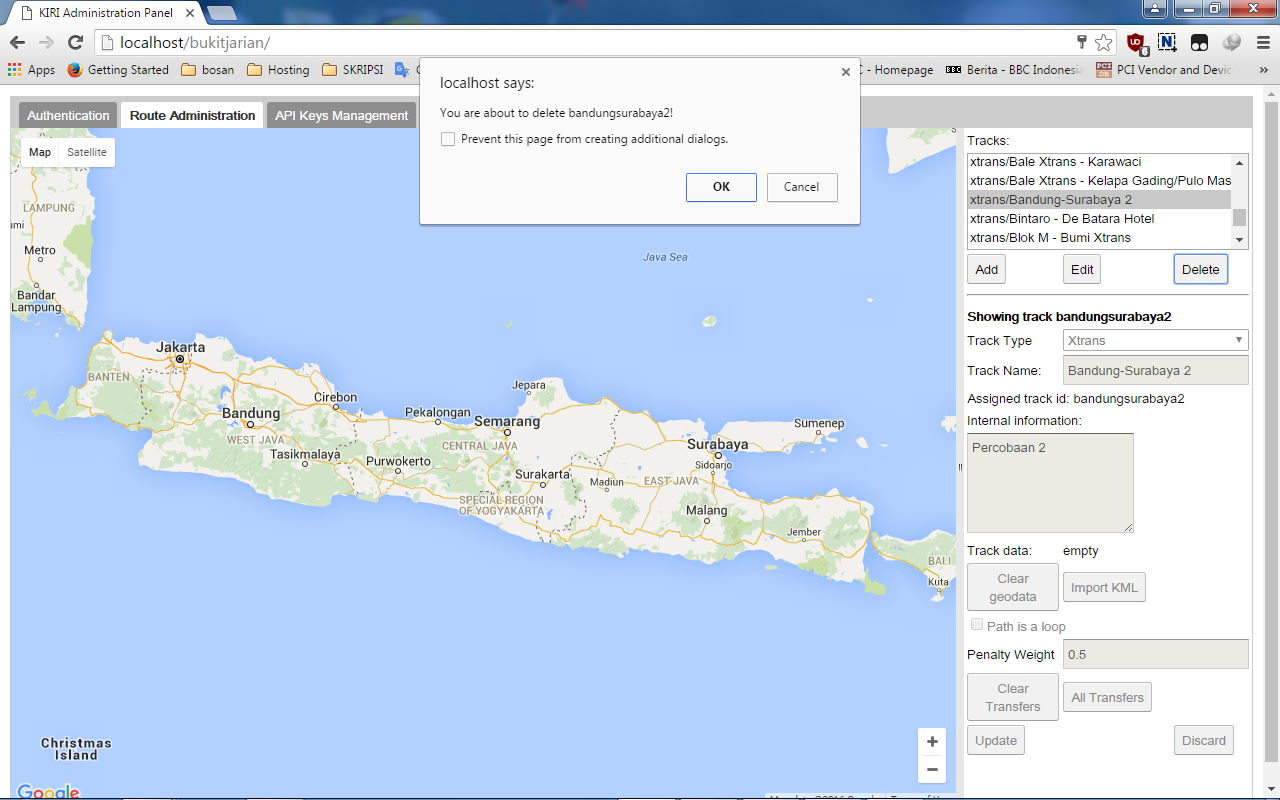
\includegraphics[scale=0.45]{Gambar/5_deletetrack_1.png}
		\caption{Memilih dan verifikasi penghapusan rute angkutan umum} 
		\label{fig:5_deletetrack_1}
	\end{figure}

	\begin{figure}[htbp]
		\centering
			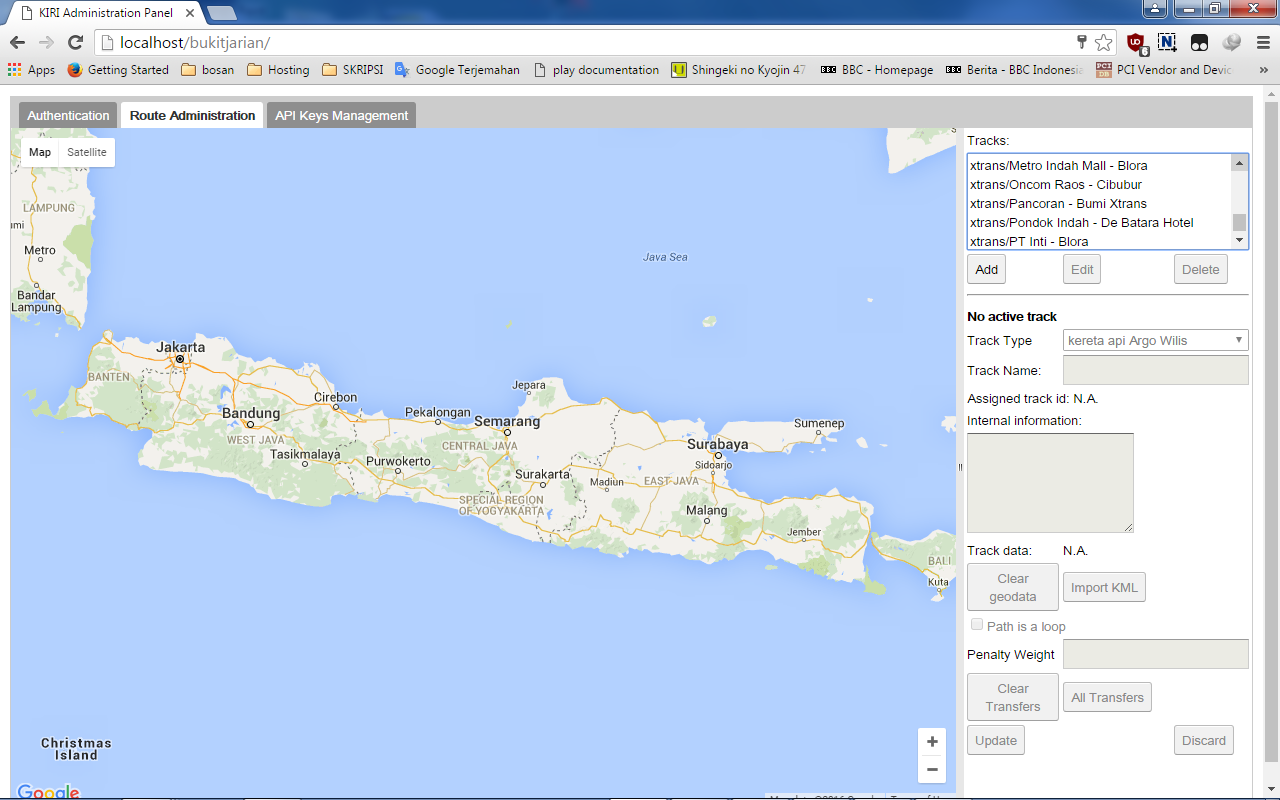
\includegraphics[scale=0.45]{Gambar/5_deletetrack_2.png}
		\caption{Rute angkutan umum hilang dari daftar} 
		\label{fig:5_deletetrack_2}
	\end{figure}

	\item \textbf{Bagian \textit{Logout}}\\
	Bagian ini merupakan bagian untuk keluar dari KIRI \textit{Dashboard}, yaitu kembali ke halaman \textit{login} (Gambar \ref{fig:5_logout}). 

	\begin{figure}[htbp]
		\centering
			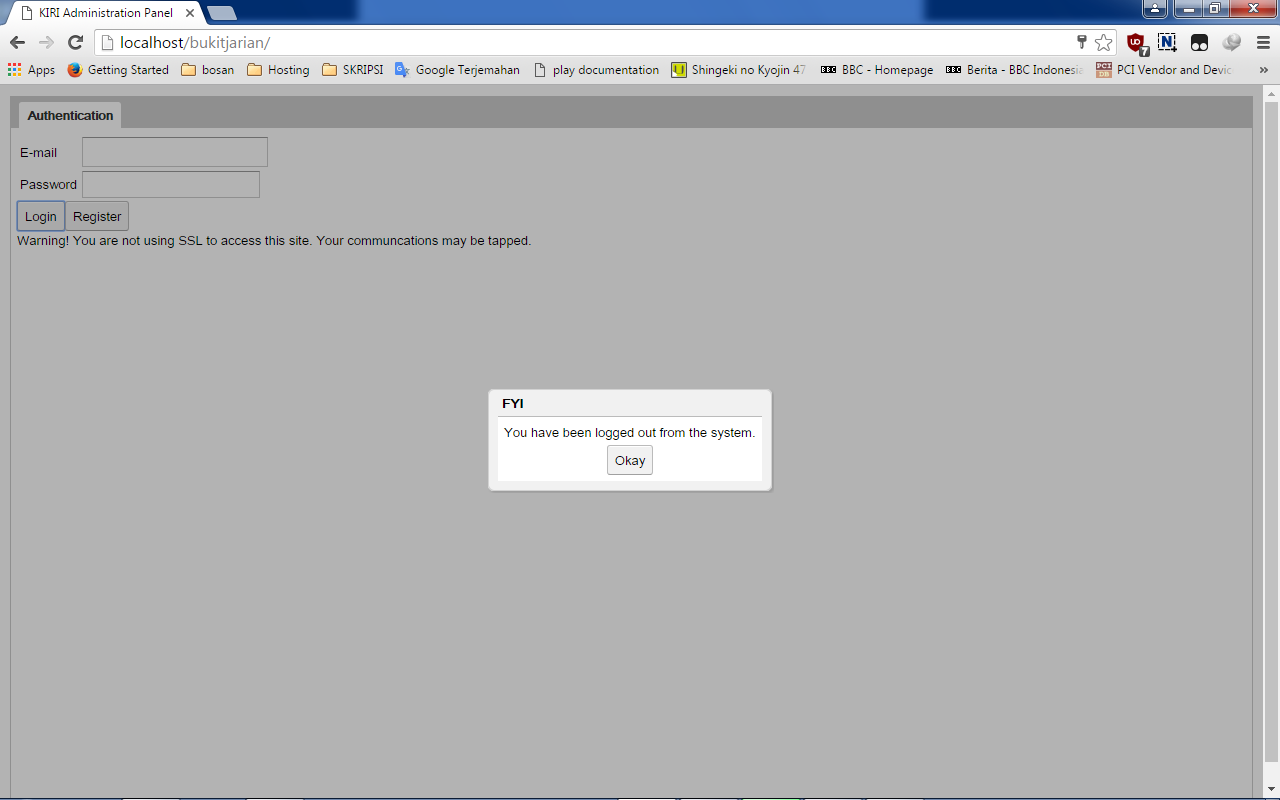
\includegraphics[scale=0.45]{Gambar/5_logout.png}
		\caption{\textit{Logout}} 
		\label{fig:5_logout}
	\end{figure}
\end{enumerate}

\section{Hasil Pengujian}
\label{sec:hasilpengujian}

\subsection{Pengujian Fungsional}
\label{sec:pengujianfungsional}
Pengujian fungsional dilakukan untuk mengetahui apakah sistem usulan sudah dapat menjalankan seluruh fungsi yang dimiliki oleh sistem kini. Pengujian ini dilakukan hanya pada sistem operasi Windows. Pengujian ini dilakukan terhadap 16 bagian sistem usulan, detail hasilnya dapat dilihat pada Tabel \ref{table:hasilfungsional}.

\begin{table}[H]
	\centering
	\caption{Tabel Pengujian Fungsional}
		\begin{tabular}{|p{0.25cm}| p{3.5cm}| p{7cm}| p{2.5cm}|} \hline
		No. & Aksi Pengguna	& Reaksi Sistem Kini & Reaksi Sistem Usulan \\ \hline
		1. & Pengguna menjalankan aplikasi & Halaman \textit{login} akan ditampilkan & sesuai \\ \hline
		2. & Pengguna melakukan \textit{register} & pengguna mendapatkan \textit{email} berupa sandi & sesuai \\ \hline
		3. & Pengguna melakukan \textit{login} & pengguna masuk ke sistem KIRI \textit{Dashboard} & sesuai	\\ \hline
		4. & Pengguna melihat data pribadi & data pribadi pengguna muncul & sesuai \\ \hline
		5. & Pengguna melihat daftar API \textit{keys} & daftar API \textit{keys} muncul & sesuai \\ \hline
		6. & Pengguna menambahkan sebuah API \textit{key} & API \textit{key} baru berhasil ditambahkan & sesuai \\ \hline
		7. & Pengguna mengubah data sebuah API \textit{key} & API \textit{key} berhasil diubah & sesuai \\ \hline
		8. & Pengguna memilih menu \textit{Route Administration} & daftar rute angkutan umum muncul & sesuai \\ \hline
		9. & dst & dst & dst \\ \hline
		\end{tabular}
	\label{table:hasilfungsional}
\end{table}

\subsection{Pengujian Eksperimental}
\label{sec:pengujianeksperimental}
Pengujian eksperimental yang dilakukan adalah pengujian terhadap waktu. Pengujian dilakukan dengan membandingkan sistem kini dan sistem usulan. Pengujian dilakukan terhadap 3 buah bagian sistem dimana setiap bagian diuji sebanyak 5 kali percobaan, detail hasil pengujian dapat dilihat pada Tabel \ref{table:hasileksperimental1} dan Tabel \ref{table:hasileksperimental2}.

\begin{table}[H]
	\centering
	\caption{Tabel Pengujian Eksperimental Sistem Kini (dalam mili sekon)}
		\begin{tabular}{|p{0.25cm}| p{7cm}| p{1cm}| p{1cm}| p{1cm}| p{1cm}| p{1cm}| p{1cm}|} \hline
		No. & Aksi & 1 & 2 & 3 & 4 & 5 & rata-rata \\ \hline
		1. & melihat data pribadi pengguna & 63 & 33 & 16 & 60 & 35 & 41.4 \\ \hline
		2. & menambahkan sebuah API \textit{key} baru & 142 & 176 & 148 & 259 & 133 & 171.6 \\ \hline
		3. & menghapus data geografi & 217 & 161 & 88 & 125 & 119 &  142\\ \hline
		\end{tabular}
	\label{table:hasileksperimental1}
\end{table}

\begin{table}[H]
	\centering
	\caption{Tabel Pengujian Eksperimental Sistem Usulan (dalam mili sekon)}
		\begin{tabular}{|p{0.25cm}| p{7cm}| p{1cm}| p{1cm}| p{1cm}| p{1cm}| p{1cm}| p{1cm}|} \hline
		No. & Aksi & 1 & 2 & 3 & 4 & 5 & rata-rata \\ \hline
		1. & melihat data pribadi pengguna & 83 & 97 & 41 & 65 & 15 & 60.2 \\ \hline
		2. & menambahkan sebuah API \textit{key} baru & 333 & 113 & 299 & 270 & 152 & 233.4 \\ \hline
		3. & menghapus data geografi & 298 & 286 & 218 & 212 & 190 & 240.8 \\ \hline
		\end{tabular}
	\label{table:hasileksperimental2}
\end{table}